

\documentclass[letterpaper, 10 pt, conference]{ieeeconf}  

\IEEEoverridecommandlockouts
%\overrideIEEEmargins
%See the \addtolength command later in the file to balance the column lengths on the last page of the document

% The following packages can be found on http:\\www.ctan.org
%\usepackage{graphics} % for pdf, bitmapped graphics files
%\usepackage{epsfig} % for postscript graphics files
%\usepackage{mathptmx} % assumes new font selection scheme installed
%\usepackage{times} % assumes new font selection scheme installed
%\usepackage{amsmath} % assumes amsmath package installed
%\usepackage{amssymb}  % assumes amsmath package installed
\usepackage{graphicx}

\title{\huge \bf
CoSTAR in Surgery: A Cross-platform User Interface \\for Surgical Robot Task Specification
}
%
\author{Baichuan Jiang, Chris Paxton, Peter Kazanzides, and Gregory D. Hager
%\thanks{$^{1}$B. Jiang is with Laboratory for Computational Sensing and Robotics, Johns Hopkins University, Baltimore, MD 21218, USA
%        {\tt\small baichuan@jhu.edu}}
\thanks{Authors are with the Department of Computer Science, Johns Hopkins University,
        Baltimore, MD 21218, USA}
%\thanks{Video demonstration can be found at https://youtu.be/RqQNLZuuRUE}
}

\begin{document}

\maketitle
\thispagestyle{empty}
\pagestyle{empty}


\newcommand{\fix}[1]{{\color{red} \textbf{[FIX: #1]}}}
\newcommand{\todo}[2]{{\color{blue} \textbf{[TODO(#1): #2]}}}

%%%%%%%%%%%%%%%%%%%%%%%%%%%%%%%%%%%%%%%%%%%%%%%%%%%%%%%%%%%%%%%%%%%%%%%%%%%%%%%%
\begin{abstract}

Human-Robot Collaboration (HRC) in surgery has been an emerging field of study in recent years, which aims at incorporating the advantages of both surgeon and machine to improve safety, accuracy and speed. In this work, we propose a cross-platform, open-source framework that would facilitate surgical HRC research. The work is based on CoSTAR, a Behavior-Tree based framework for end-user instruction of industrial robots~\cite{paxton2017costar}. To demonstrate its feasibility as a platform for collaborative surgical robot research, we generalized the original system and implemented it on the da Vinci Research Kit (dVRK), while maintaining its full functionality on other robot platforms such as UR5 and KUKA LBR iiwa.  

\end{abstract}


%%%%%%%%%%%%%%%%%%%%%%%%%%%%%%%%%%%%%%%%%%%%%%%%%%%%%%%%%%%%%%%%%%%%%%%%%%%%%%%%
\section{Introduction}

Surgical robots have been increasingly adopted in clinical procedures to support surgeons with various tasks, although most systems currently available are under full control of the surgeon. It is suggested in recent studies \cite{padoy2011human,berthet2016hubot,bauzano2016collaborative,hu2015semi} that incorporating further intelligence into the surgical robot will free surgeons from repetitive tasks, reduce large movements of the master manipulator to avoid frequent clutching and readjusting hand position, and achieve better overall precision and accuracy. 

Many proposed collaborative schemes aim to take advantage of the reliability that robots offer when performing less critical tasks, while taking advantage of the surgeons' domain knowledge to perform fine manipulation actions. Padoy \textit{et al.}~\cite{padoy2011human} adopted a Hidden Markov Model (HMM) as a way of modeling a surgical procedure in order to automatically alternate between manual and automated subtasks. Hubot~\cite{berthet2016hubot} system runs continuously in a loop alternating between fully manual, manual with haptic guidance, and fully automated modes. This kind of ``human decide, robot do'' scheme was also used in semi-autonomous brain tumor ablation \cite{hu2015semi}.

%Therefore, we propose a common task specification framework where tasks can be represented by nodes of behavior tree, corresponding to different phases in these collaborative schemes. The user can easily construct a Behavior Tree to automate parts of the procedure to adapt it to their specific scenarios. 

%Collaboration system for HALS procedure \cite{bauzano2016collaborative} where surgeon inserts a hand into abdomen while operating the laparoscopic instrument using the other hand also utilizes a workflow manager to allow the robot being informed of the current state of intervention.

CoSTAR~\cite{paxton2017costar} aims to do something similar for collaborative robots but provides further extensibility than purely ontology-based system. 
%This work is a surgical generalization of our previous work in \cite{paxton2017costar}, where the aim is to provide an easy way of authoring task plans for industrial robots such as UR5 and KUKA LBR iiwa.
CoSTAR's core features are a modular architecture that combines planning, perception, and logic via a Behavior Tree-based task specification UI, previously shown on the KUKA LBR iiwa and the Universal Robots UR5. Here, we propose to adapt and expand the system to make it suitable for surgical robotics, where an expert user can construct a Behavior Tree to automate parts of the procedure and adapt it to their specific scenarios.
The system setup is shown in Fig.~\ref{fig:dvrk}. 

\begin{figure}[bt]
\centering
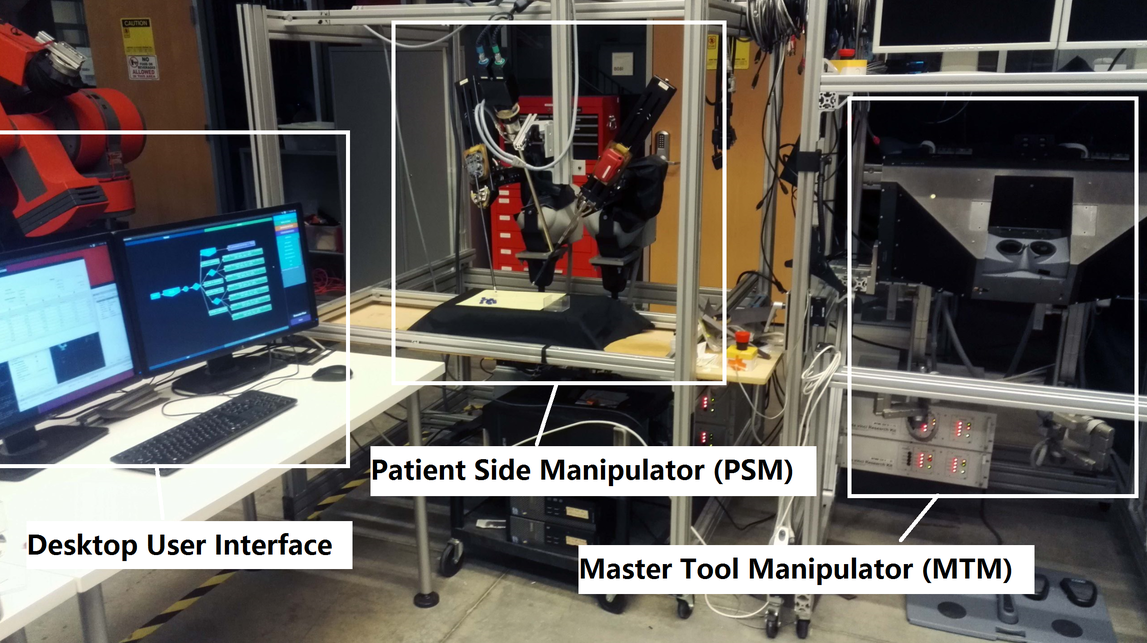
\includegraphics[width=240pt]{dvrk.png}
\caption{CoSTAR implementation on dVRK. Users design the task plan using the user interface on the screen to the left, and then use the master console on the right to perform manual portions of the procedure.}
\label{fig:dvrk}
\end{figure}


\section{System Architecture}
%\subsection{Component based framework}
A modular framework is one key for cross-platform implementation. CoSTAR is composed of a set of modular \textit{Components}, such as \texttt{GRIPPER} and \texttt{ARM}. Each component $C$ is associated with a set $(I,O,s,p,u)$: 

\begin{itemize}
\item \textit{Input $I$ and Output $O$} are represented by ROS topics and they are never explicitly exposed to the end-user. 
\item \textit{Symbols $s$} are populated from input as a function of the raw state of the world, which represent objects and positions, such as \texttt{LEFT OF} or \texttt{PRESSED}.
\item \textit{Predicates $p$} describe the quality of existing symbols or their relationship, which is more formally expressed as a function mapping $p(I,s_0, ..., s_n) \rightarrow [\texttt{TRUE}, \texttt{FALSE}]$ that can be used to control workflow. 
\item \textit{Operations $u$} are the specific actions that would change the value of stored symbols or the state of the robot. 

\end{itemize}

Another key for modularity is the inheritance within each component. For example, components \texttt{PSM} and \texttt{DVRK\char`_GRIPPER} for the patient side manipulators are instantiations spawned from the abstract component \texttt{ARM} and \texttt{GRIPPER} by implementing the required functionalities such as \texttt{MOVE} and \texttt{CLOSE\char`_GRIPPER}. More detailed description of components can be found in \cite{paxton2017costar}.

\subsection{Behavior tree instructor interface}

%To enable cross-platform implementation, a modular framework is designed. Taking the component \texttt{ARM} as an example, the inheritance within each component is the key part of the modularity. The abstract component \texttt{ARM} provides a list of functionalities, and all undefined but required functionalities such as \texttt{TEACH} and \texttt{MOVE} must be implemented by a particular instantiation of \texttt{ARM}, resulting in components \texttt{UR}, \texttt{IIWA}, and \texttt{PSM}. 
%
%Each component $C$ can be viewed as a set $(I,O,p,s,u)$ that associates with input data $I$, output data $O$, set of predicates $p$, set of symbols $s$ and set of operations $u$. Input and output are represented by ROS topics. Symbols represent abstract objects like \texttt{LEFT OF} (vision) or \texttt{PRESSED} (button), and predicates describe the qualities of these objects, which map symbols to a Boolean and can be used as start/stop conditions to control task workflow. More details of the component definition can be found in \cite{paxton2017costar}.
%
%Basic components for CoSTAR system task execution such as \texttt{Perception}, \texttt{Gripper}, \texttt{Arm} and \texttt{Predicator} are united by behavior-tree based component \texttt{Instructor}. Symbols and predicates produced by components such as \texttt{Perception}, \texttt{Gripper}, \texttt{Arm} are aggregated by \texttt{Predicator} which controls the task workflow of the behavior tree. 

A behavior tree is expressive to represent a great variety of tasks accommodating different scenarios for human-robot collaborative surgery. This is achieved through the linking of internal nodes:
 
\begin{itemize}
\item \texttt{SEQUENCE} node: tick each child in order, until each one reports \texttt{SUCCESS}. One child's fail will result in the sequence's fail.
\item \texttt{SELECTION} node: tick each child in order until one returns success.
\item \texttt{REPEAT N} node: tick children until N successes or failures are reported.
\item \texttt{RESET N} node: returns the value of child, but resets the child up to N times.
\end{itemize} 

We can combine these structural and operation nodes to create a behavior tree that encapsulates very complex behavior. The process of creation can be greatly simplified using the \texttt{INSTRUCTOR} user interface as shown in Fig. \ref{fig:instructor}.

\begin{figure}[bt]
\centering
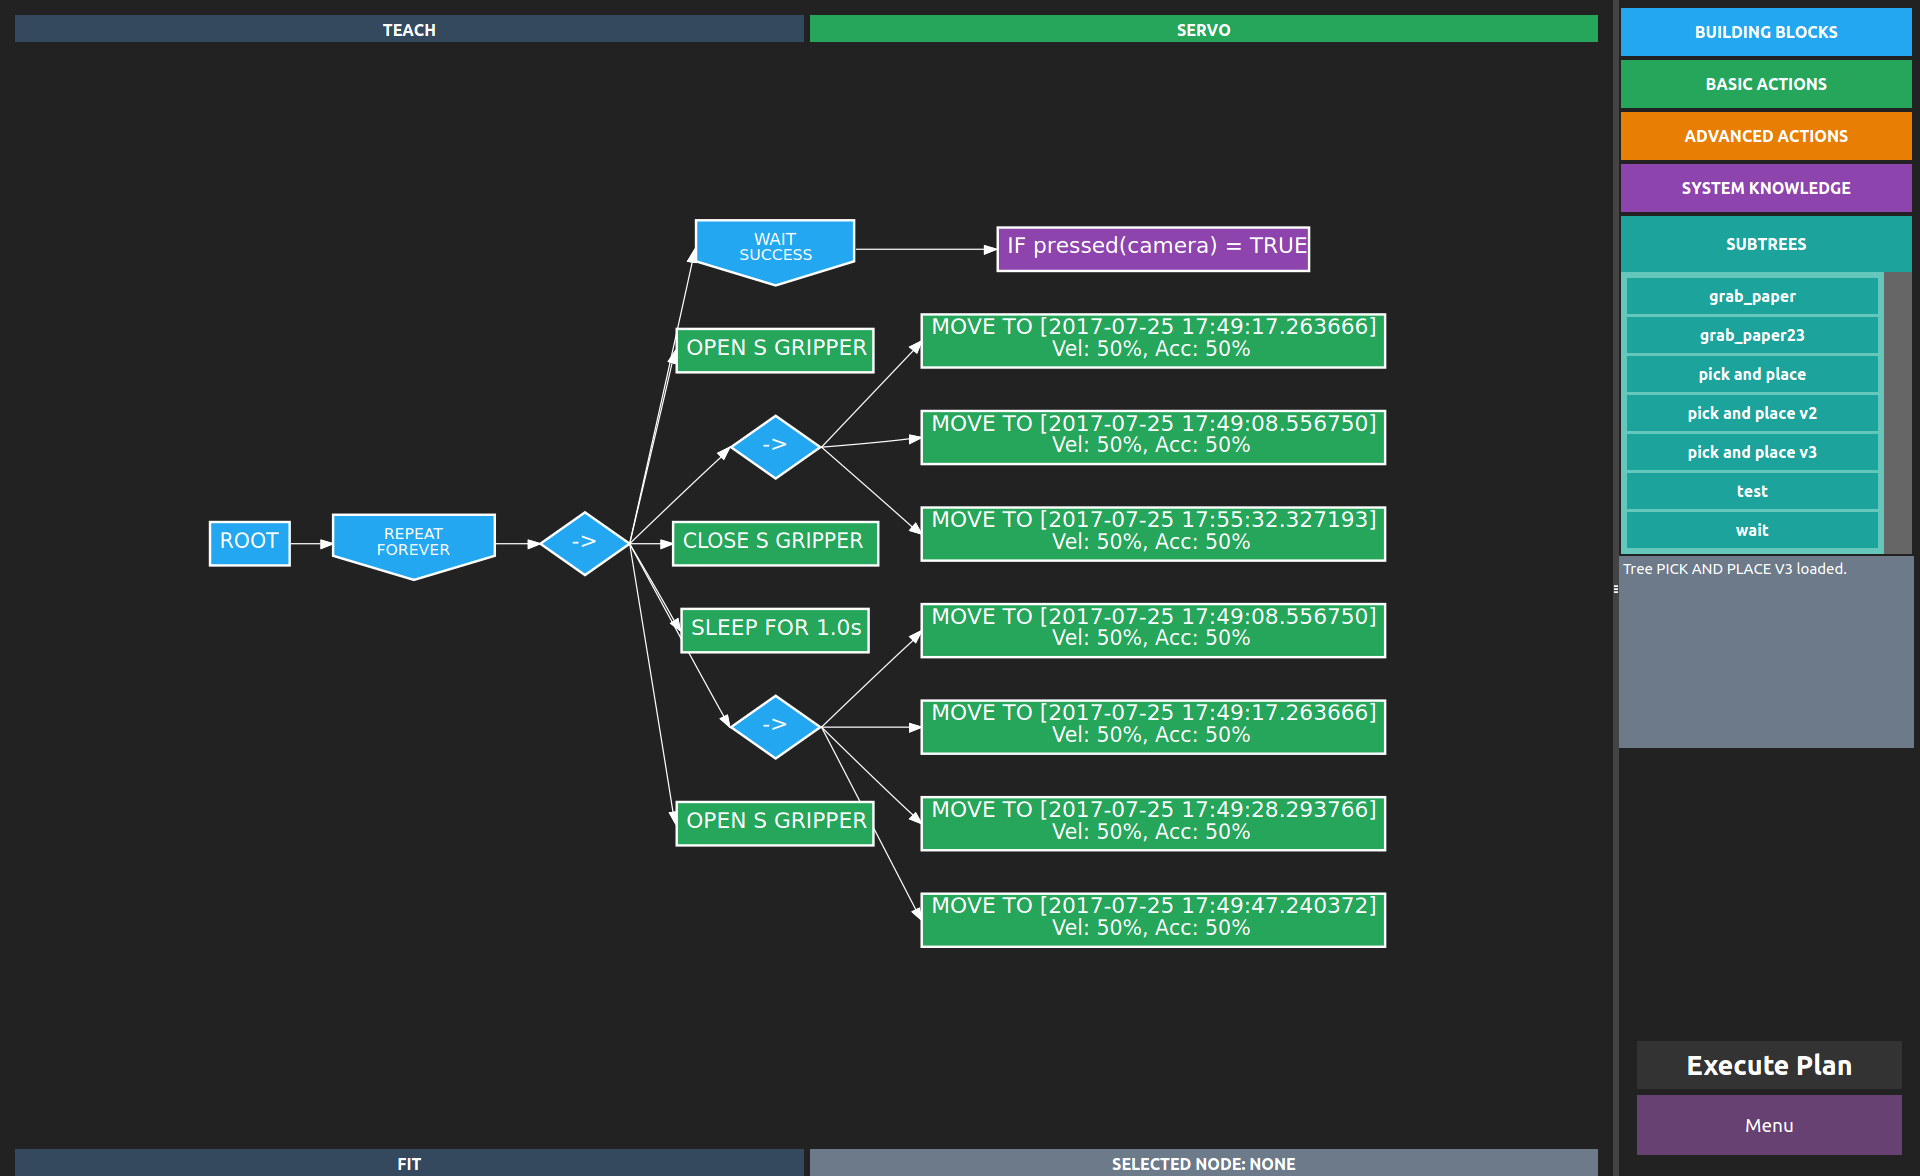
\includegraphics[width=240pt]{instructor2.png}
\caption{CoSTAR \texttt{INSTRUCTOR} user interface: tabs on the right have different functionalities to build a behavior tree and are able to do subtree manipulation. }
\label{fig:instructor}
\end{figure}


\section{Case Study}
A simple surgical scenario where the framework will be helpful and easy to use is \textit{debridement}, which involves removing the dead tissue fragments during surgical treatment. We set up the experiment \cite{video} as in Fig. \ref{fig:dvrk} and Fig. \ref{fig:debridement}. 

The target in this experiment is to transfer the pile of debridements  on the left to the tray on the right. Because it is safer to set the motion scale at a low level during teleoperated robotic surgery, the workspace of the dVRK Patient Side Manipulator (PSM) is limited and requires frequent clutching of the Master Tool Manipulator (MTM) to reorient the slave workspace. Therefore, we propose a two-step procedure: first use PSM1 (left) to manually pick one fragment to a fixed position, then let PSM2 (right) to automatically pick it up and place it in the tray. The second step can be achieved through a learn-from-demonstration (LfD) scheme: first the surgeon demonstrates the pick-and-place procedure while recording waypoints during manipulation. The saved waypoints that follow a safe path can be used to automate the robot during the second step. 

The above procedure can be represented by a behavior tree as shown in Fig. \ref{fig:instructor}. The execution order for our user interface is from left to right and from top to bottom. Following the \texttt{ROOT} node, a \texttt{REPEAT} node is set to repeat the per-fragment action. Then a \texttt{SEQUENCE} node follows, representing the automation sequence. The \texttt{PREDICATOR} node for pedal press signal is set after the \texttt{WAITFORSUCCESS} node, so that the workflow proceeds whenever the pedal is pressed. Finally, operation nodes such as \texttt{OPENGRIPPER} and \texttt{MOVETOWAYPOINTS} complete the full procedure. 

By automating the PSM2 pick-and-place, the surgeon can focus on using PSM1 to place the debris at the fixed location under a safer motion scale. Whenever triggered by a pedal press, PSM2 will repeat the action so that two arms can be operated at the same time, thus greatly increasing the speed.  


\begin{figure}[bt]
\centering
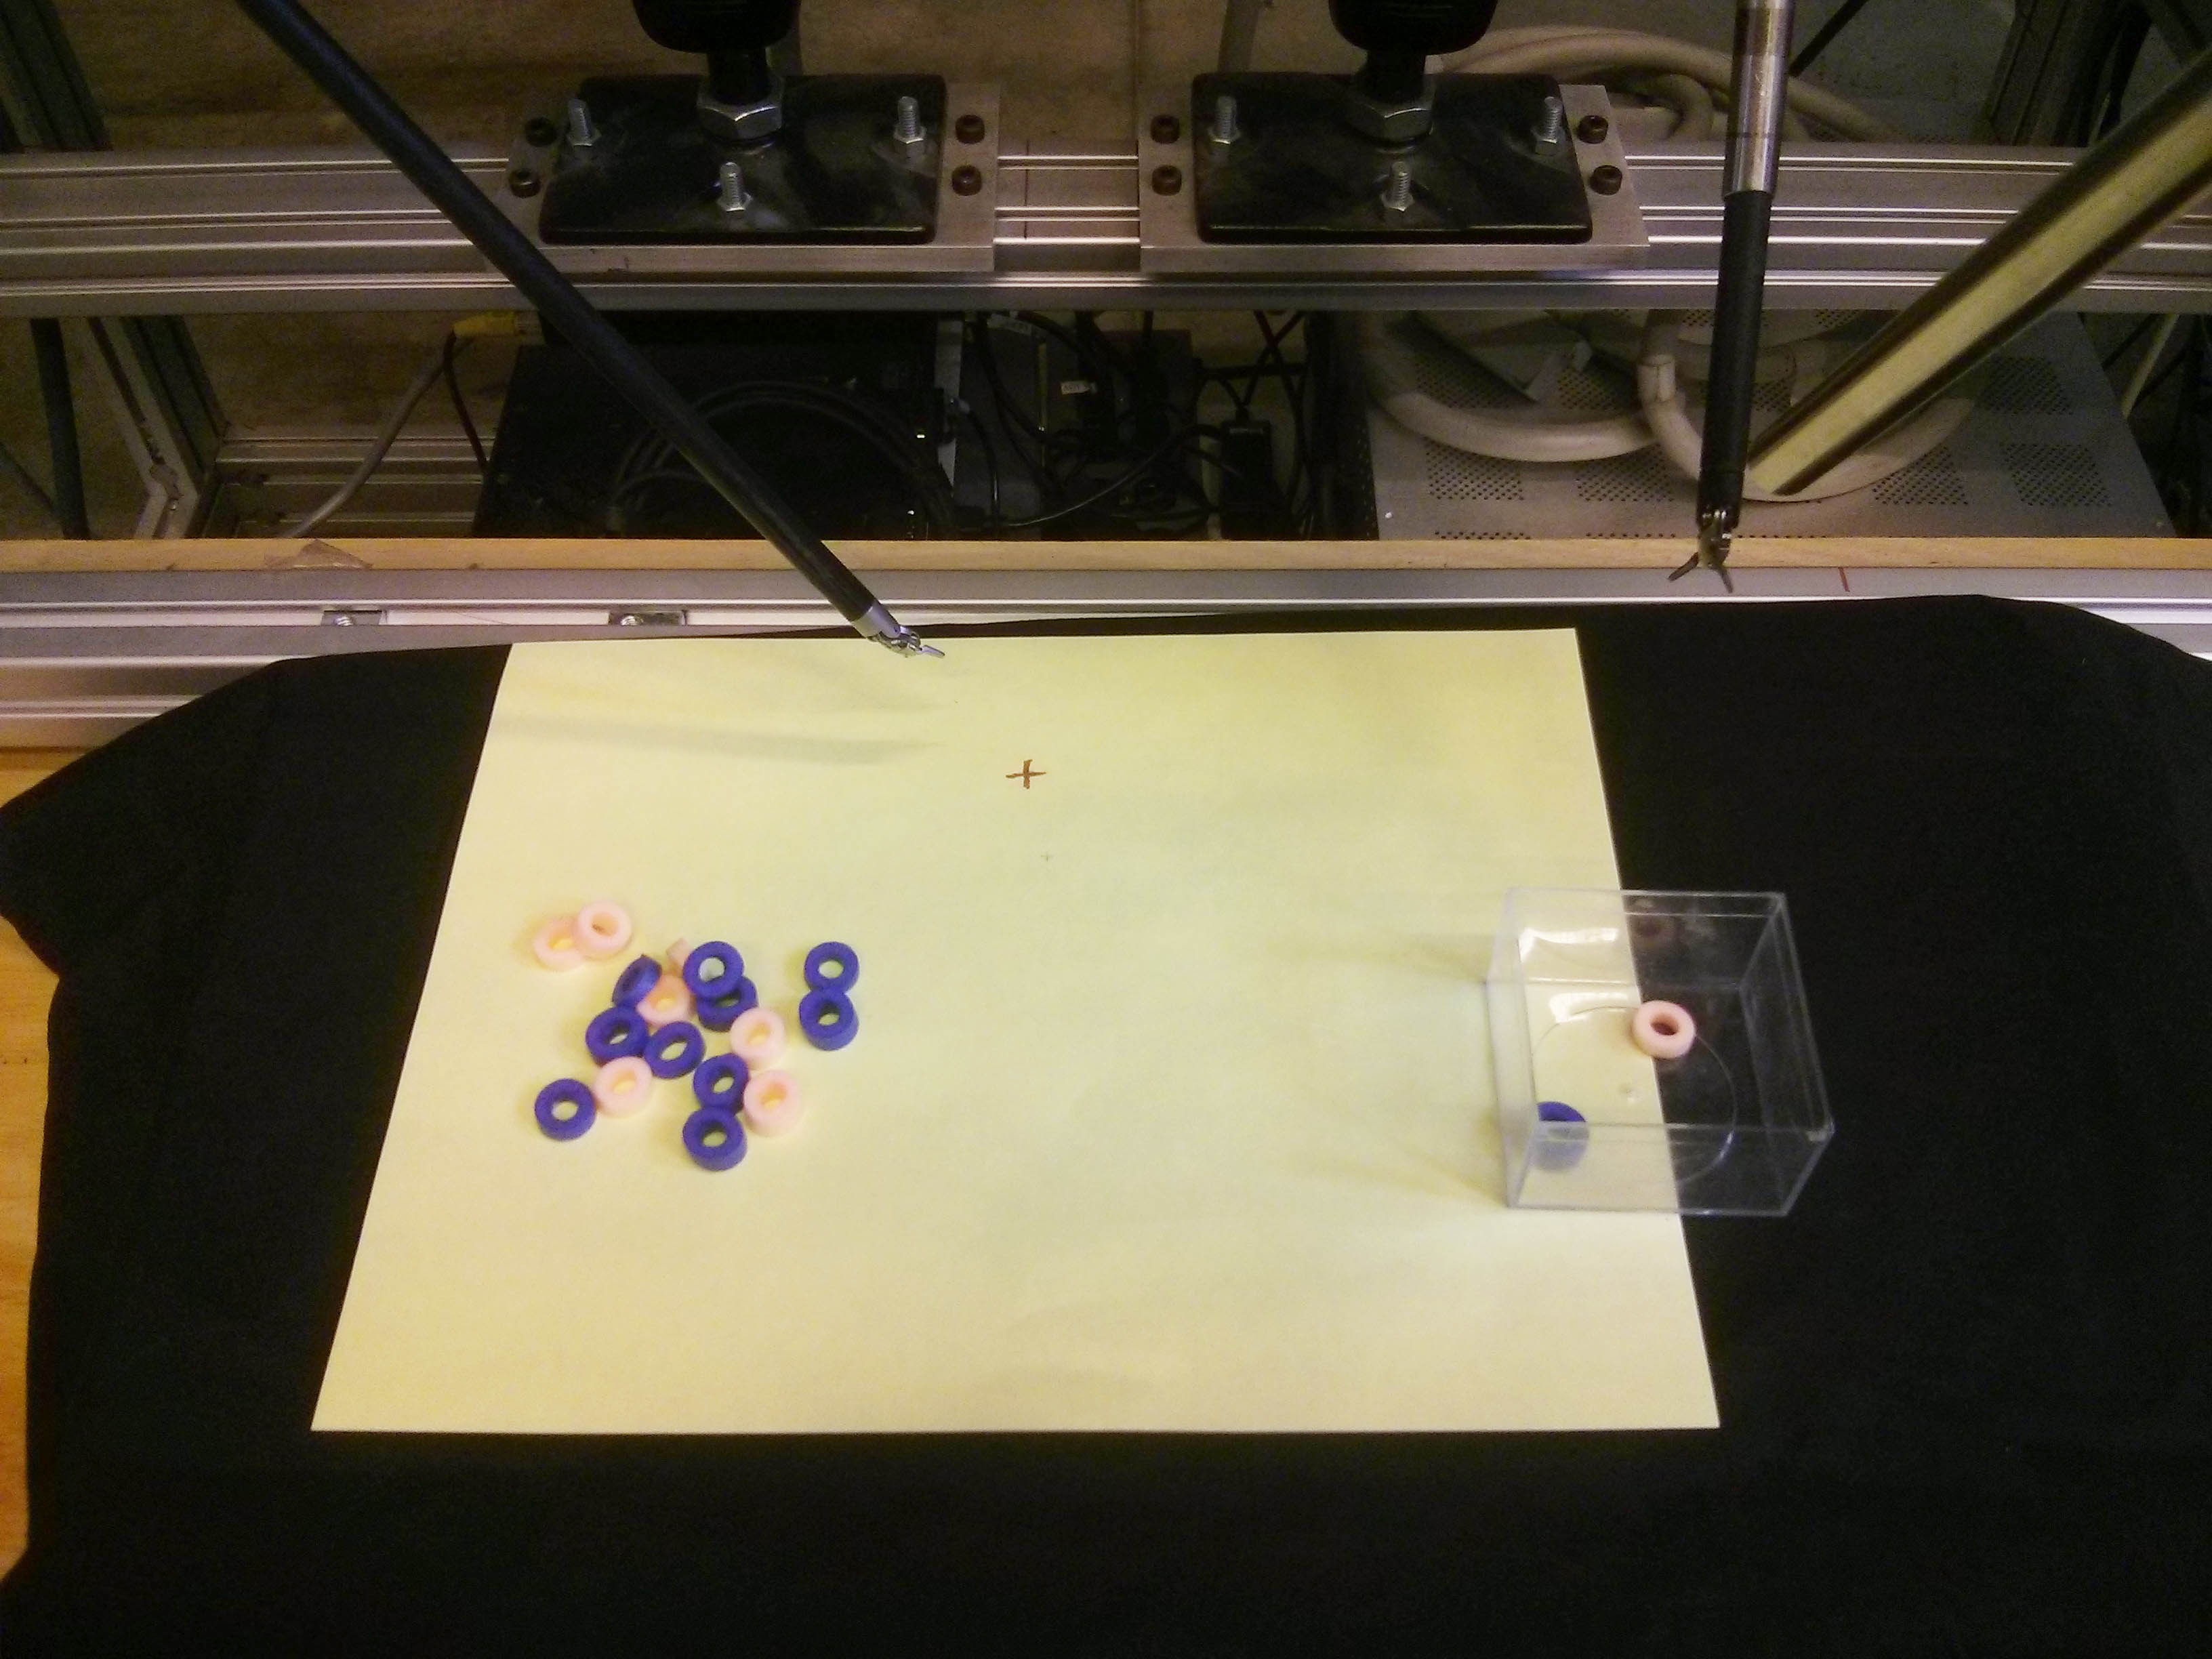
\includegraphics[width=195pt]{debridement.jpg}
\caption{Debridement experiment setup. PSM1 will pick one debris from the left pile and place it on the red cross, then PSM2 will pick the piece from the red cross and transport it to the tray.}
\label{fig:debridement}
\end{figure}


\section{Conclusion}
The modular framework and abstract representation of workflow and environment state (by predicates and symbols) make the proposed system ideal surgical HRC platform. Emerging topics such as machine learning based action detection or vision based surgical robot automation can be easily incorporated in this framework as a component. 

For the proposed system itself, it allows surgeons to easily author task plans for various scenarios with an appropriate level of automation. This will be of great benefit when multiple robot arms are present (such as a full da Vinci Surgical System) or in a Hand-Assisted Laparoscopic Surgery (HALS) procedure \cite{bauzano2016collaborative} where the surgeon only has one free hand to operate multiple tools. 


\addtolength{\textheight}{-12cm}   % This command serves to balance the column lengths
                                  % on the last page of the document manually. It shortens
                                  % the textheight of the last page by a suitable amount.
                                  % This command does not take effect until the next page
                                  % so it should come on the page before the last. Make
                                  % sure that you do not shorten the textheight too much.

%%%%%%%%%%%%%%%%%%%%%%%%%%%%%%%%%%%%%%%%%%%%%%%%%%%%%%%%%%%%%%%%%%%%%%%%%%%%%%%%



%%%%%%%%%%%%%%%%%%%%%%%%%%%%%%%%%%%%%%%%%%%%%%%%%%%%%%%%%%%%%%%%%%%%%%%%%%%%%%%%



%%%%%%%%%%%%%%%%%%%%%%%%%%%%%%%%%%%%%%%%%%%%%%%%%%%%%%%%%%%%%%%%%%%%%%%%%%%%%%%%
%\section*{APPENDIX}
%
%\section*{ACKNOWLEDGMENT}


%%%%%%%%%%%%%%%%%%%%%%%%%%%%%%%%%%%%%%%%%%%%%%%%%%%%%%%%%%%%%%%%%%%%%%%%%%%%%%%%

%References are important to the reader; therefore, each citation must be complete and correct. If at all possible, references should be commonly available publications.

\bibliographystyle{IEEEtran}
\bibliography{surgical}

\end{document}
